\chapter{TCP IP}


\section{分层}


\section{主要协议基本介绍}


\section{以太网数据报}

\section{IP数据报}


\section{ARP RARP}

\section{ICMP}


\section{IP路由}

\subsubsection{选路原理}
\begin{enumerate}
\item 搜索匹配的主机地址;
\item 搜索匹配的网络地址;
\item 搜索默认表项
\end{enumerate}
\subsubsection{路由表}


Flags
\begin{itemize}
\item U 该路由可以使用
\item G 该路由是一个网关(路由器),如果没有这个标志,说明目的地是直接相连的

这个标志的重要性,他区分了间接路由和直接路由(直接路由不设置标志G)。区别是发往直接路由的分组中不但具有指明的目的IP地址,还具有其链路层地址。而对于间接路由,IP地址指明的是最终目的地,但是链路层地址指明的是网关(即下一站路由器)。

这里我的理解是。对于同一个局域网的主机,只需要一条记录,就是网络号的部分,然后所有主机都使用这一条记录,所以IP数据报发送出去的目的和链路层都是目的主机的。

\item H 该路由是到一个主机
\item D
\item M
\end{itemize}

如果没有默认路由,没有找到匹配项的情况下,如果是本机产生的,就给应用程序返回一个差错:或者主机不可达,或者网络不可达错。
如果是转发的数据报,那么就给原始端发送一份ICMP主机不可达差错报文。

一般主机不转发数据报,除非对他们进行了设定作为路由器使用。

\paragraph{ICMP重定向}
\begin{enumerate}
\item 主机发送一份数据报到R1,比如因为R1是默认主机;
\item R1接收到数据报并且检查路由表,发现R2是发送该数据报的下一站,当他把数据报发送到R2是,发现接收和发送的接口是相同的(即主机和两个路由器所在的LAN),这样就给路由器发送重定向报文给原始发送端提供了线索
\item R1发送一份ICMP重定向报文给主机,告诉他以后数据报发送给R2而不是R1
\end{enumerate}

%此处需要插入图片

生成ICMP重定向报文的条件:
\begin{itemize}
\item 出口和入口相同
\item 用于向外传送数据报的路由不能被ICMP重定向报文创建或者修改,而且不能是路由器的默认路由;
\item 数据报不能用源站选路来转发
\item 内核必须配置成可以发送重定向报文
\end{itemize}

接收重定向报文的主机必须确定满足下面条件才能修改路由表
\begin{itemize}
\item 新的路由器必须直接与网络相连接
\item 重定向报文必须来自当前到目的地所选择的路由器
\item 被修改的路由器必须是一个间接路由
\end{itemize}

\paragraph{ICMP路由器发现报文}

\subsubsection{动态选路协议}
相邻的路由器之间通信,以告诉对方每个路由器当前所连接的网络。

RIP(选路信息协议)

RIP报文包含在UDP数据报中,常用的UDP端口为520.

报文格式:

\begin{itemize}
\item 初始化

在启动一个路由守护进程时,先判断启动了哪些接口,并在每个接口上发送一个请求报文,要求其他路由器发送完整路由表。

命令字段为1,度量为16(特殊请求,要求对方发送完整路由表的请求)。

\item 接收响应,如果是上面的特殊请求,则发送完整路由表,否则处理请求中的每一个选项,如果有连接,则指明连接到目的地的路由,将度设定为我们的值,否则设定为16(表示无穷大),然后响应。

\item 定期更新,每个30秒,所有或者部分路由会将其完整路由表发送给相邻的路由器。广播形式。

\item 触发更新 当一条路由的度发生变化时,就对他进行更新,只发送发生变化的项。

每条路由都有与之相应的计时器,如果运行RIP的系统发现一条路由3分钟内未更新,则将该路由设置为无穷大(16),并且标注为删除,再过60秒,在本地路由表中删除该路由,以保证该路由表的失效已被传播开。

\end{itemize}

缺陷,没有子网概念。



\section{UDP}

\subsubsection{UDP数据报}

封装成IP数据报的格式。

%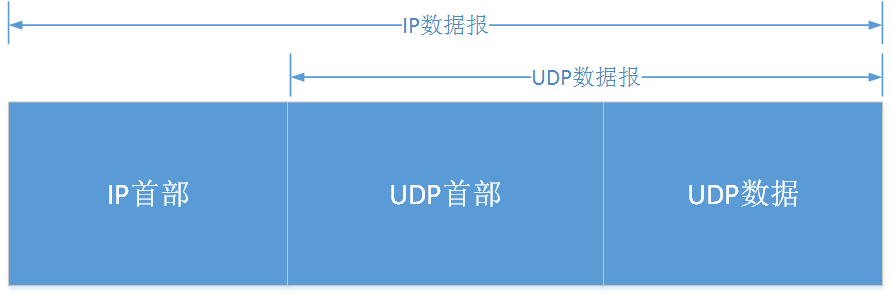
\includegraphics[scale=0.5]{protocol/resources/UDP数据报.png}


\subsubsection{UDP首部}

16位源端口,16位目的端口,16位UDP长度(首部+数据,最小8字节),16位UDP校验和

\subsubsection{IP分片}

\begin{itemize}
\item IP层收到一份要发送的数据报时,要判断向本地的哪个接口发送,并查询该接口获得他的MTU。比较数据报长度和MTU,如有需要就进行分片。

\item 可以在原始主机或者中间路由进行分片

\item 一份IP数据报分片后,只能在目的主机才进行重新组装

\item IP首部标识字段都包含维一值,该值在分片时被复制到每一个分片,用其中1bit来表示是否有更多分片,除最后一个分片,其他都被置成1.片偏移字段表示偏离原始数据开始位置。

\item 标示位有1bit表示“不分片”,如果这个位被置为1,则要分片时不进行分片,丢弃数据并返回一个ICMP错误报文。

\item 分片丢失需要重传整个IP数据报
\end{itemize}

\subsubsection{ICMP(需要分片)}

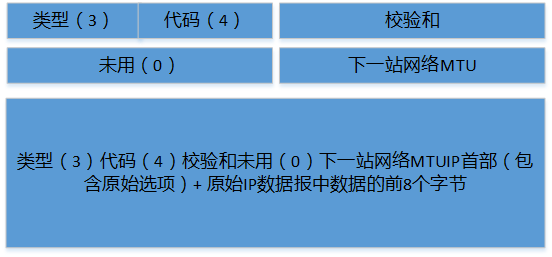
\includegraphics[scale=1]{protocol/resources/ICMP-header.png}

如果路由不能提供这种新格式的ICMP,则下一站MTU设置0。

\subsubsection{Traceroute确定路径MTU}

设置不可分片,最开始使用出口的MTU,当收到ICMP不可分片差错时,如果是最新的ICMP报文,就包含下一站最小MTU,则使用这个MTU来发送,否则,使用下一个可能的MTU(RFC1191声明可用的MTU个数是有限的)

\subsubsection{UDP服务器设计}



\section{广播和多播}

\subsection{广播}

四种广播地址

\subsubsection{受限的广播地址}

255.255.255.255,用于网络配置过程中IP数据报的目的地址,此时,主机可能还不知道主机所在网络的网络掩码,可能主机连IP地址都不知道。

路由不转发目的地址为受限广播地址的数据报。

\subsubsection{指向网络的广播地址}

\subsubsection{指向子网的广播地址}

\subsubsection{指向所有子网的广播地址}

\subsection{多播}



\section{TCP}

\subsection{首部}

\begin{itemize}
\item 应用数据被分割成TCP认为最合适发送的数据块
\item TCP发送一个段后,启动一个定时器,等待目的地确认接收到这个段,如果不能及时收到确认,则重传。
\item TCP收到另一端的数据后,会发送一个确认,不会立即发送,而是延时几分之一秒
\item TCP通过IP传送,到达可能失序,TCP会重新排列之后,将数据发送给应用程序。
\item TCP提供流量控制

\end{itemize}


一个IP地址加一个端口也称为socket。插口对(socket pair) (包含客户IP地址、客户端口号、服务器 IP地址和服务器端口号的四元组 )可唯一确定互联网络中每个TCP连接的双方。

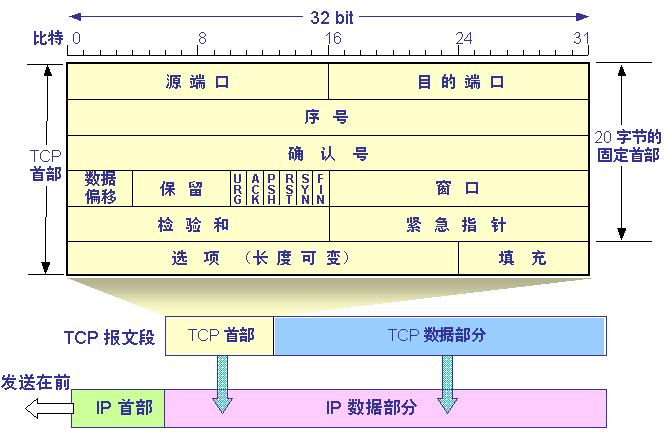
\includegraphics[scale=3]{protocol/resources/TCP-header.jpg}


\begin{itemize}
\item 序号,TCP用序号对每个字节计数,32bit无符号数,表示这个报文中第一个数据字节。到达$2^{32} - 1$之后重新从0开始。最开始的值为ISN,然后SYN占掉1位,所以第一个TCP数据段的序号是ISN+1。

\item 数据偏移(首部长度),因为有可变长度的选项。最小20字节,没有选项,最大60字节。

\end{itemize}

\subsection{建立和终止连接}

\subsubsection{建立连接}

\begin{enumerate}
\item 请求段发送一个SYN段指明客户端打算连接到服务器的端口,以及初始序列(ISN);

\item 服务器发回包括服务器初始ISN的报文段作为应答,同时将确定序号设置为客户的ISN+1以对客户端的SYN报文段进行确认;

\item 客服端将确认序号设置为服务器ISN+1,用来对服务器的SYN进行确认。

\end{enumerate}

\subsubsection{终止连接}

建立连接由3次握手完成,二断开连接需要经过4次握手。TCP连接是全双工,因此需要每个方向单独关闭。

\begin{enumerate}
\item 客服端发送一个FIN,服务器响应一个ACK,确认序号为客服端的序号+1

\item 服务器发送一个FIN,客服端响应一个ACK,确认需要为服务器的序号+1
\end{enumerate}

